\chapter{测试与评估}

本章将介绍面向Hyperledger Fabric的区块链云化框架的测试与评估工作。首先, 本章以典型案例的方式对原型工具进行测试;其次, 采用SAAM、定性与定量方法\cite{tashakkori1998mixed}结合五层成熟度模型以及与官方工具Cello\footnotemark[1]\footnotetext[1]{\href{https://github.com/hyperledger/cello}{Hyperledger Cello}}进行对比评估。



\section{测试环境}

为全面对本文提出的区块链云化框架与工具进行测试, 本文对原型工具进行了功能性测试、场景分析以及工具对比测试, 由于在本机环境下搭建Cello会出现诸多问题, 如文件挂载权限、编译等, 所以本文准备了两套测试环境。本文首先在本地环境进行功能方面的测试, 本地机器为MacBook Pro, 并采用Docker for Desktop搭建的单节点Kubernetes充当集群环境; 其次, 在第\ref{section: tool_comparison}节中, 为顺利运行对比工具Cello, 本文利用云主机Ubuntu 18.04搭建Minikube充当集群环境。上述两种环境具体配置如表\ref{computer}所示。

{\footnotesize
\begin{longtable}[h]{m{40pt}|m{100pt}|m{100pt}}
    \caption[配置详情]{配置详情} \label{computer} \\
        \hline   
        \textbf{环境}&\textbf{配置项目}&\textbf{配置详情}\\
        \hline
        \multirow{2}*{\parbox[c]{40pt}{本机环境}}    
        & Docker for Desktop&Version 4.7.0\\     
        & Kubernetes&v1.22.5\\
        \hline
        \multirow{3}*{\parbox[c]{40pt}{云主机}} 
        & Docker & Community 20.10.13 \\
        & minikube & v1.25.2 \\
        & Kubernetes & v1.23.3 \\
        \hline 
    \end{longtable} 
}


\section{原型工具测试}\label{section: tool_test}

本小节主要以案例分析的形式对原型工具进行功能性测试。如图\ref{fabric_net}所示, 本节将以搭建最经典、简单的HF网络案例的方式针对\ref{section: requirement}节的用例进行完整的功能测试。测试重点针对于Ca、Peer、Orderer启动、创建通道、部署链码的全部过程, 验证HF网络启动及链码部署的正确性。

\begin{figure}[h] %figure环境,h默认参数是可以浮动,不是固定在当前位置。如果要不浮动,你就可以使用大写float宏包的H参数,固定图片在当前位置,禁止浮动。
    \centering %使图片居中显示
    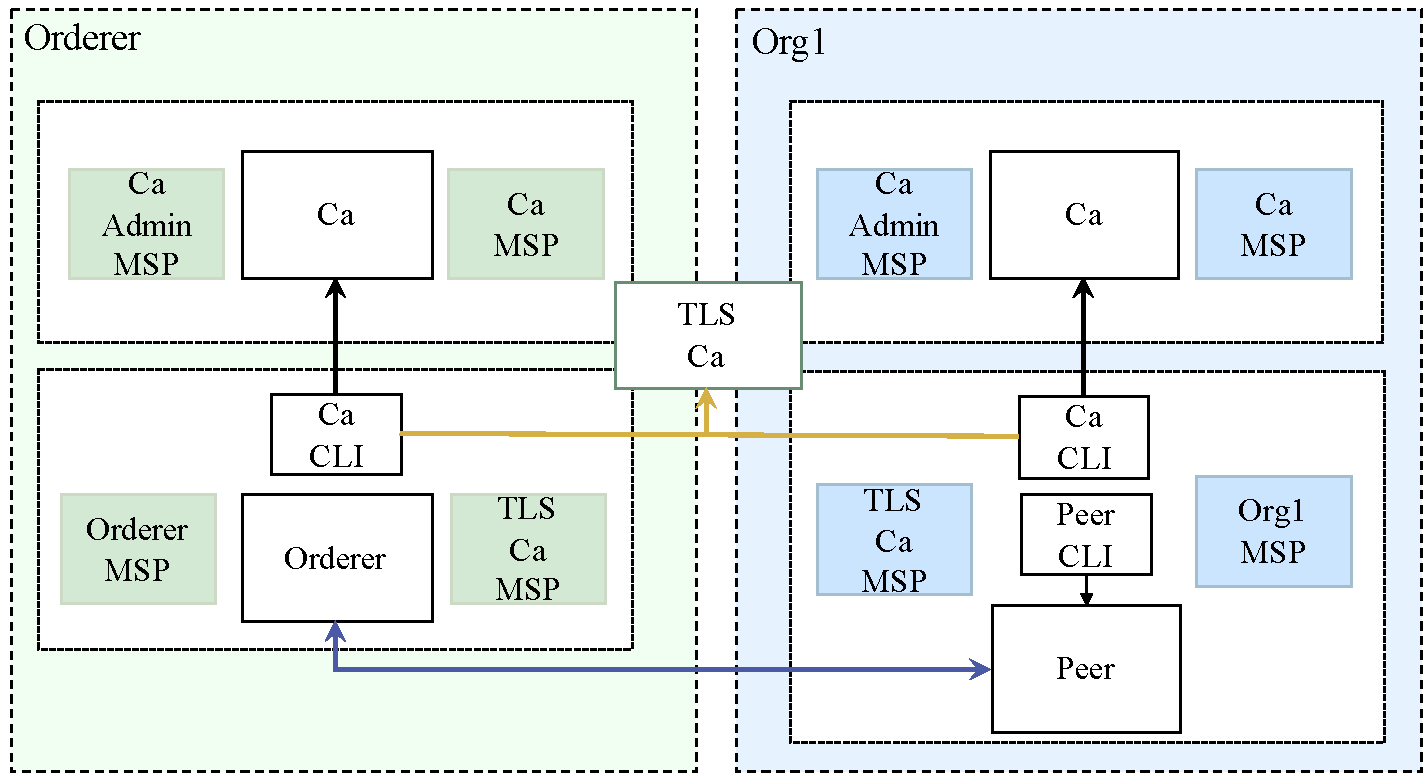
\includegraphics[width=1.0\textwidth]{FIGs/chapter5/fabric_net.pdf} %中括号中的参数是设置图片充满文档的大小,你也可以使用小数来缩小图片的尺寸。
    \caption{测试网络} %caption是用来给图片加上图题的
    \label{fabric_net} %这是添加标签,方便在文章中引用图片。
\end{figure}%figure环境

\textbf{前置条件:}原型工具首先将编写好的HF网络各节点的CRDs注入Kubernetes。注入的CRDs可以通过原生kubectl命令进行管理。如图\ref{crdresult}所示为部署之后的结果, 已经将Ca、Peer、Orderer的CRD部署入集群。

\begin{figure}[h] %figure环境,h默认参数是可以浮动,不是固定在当前位置。如果要不浮动,你就可以使用大写float宏包的H参数,固定图片在当前位置,禁止浮动。
    \centering %使图片居中显示
    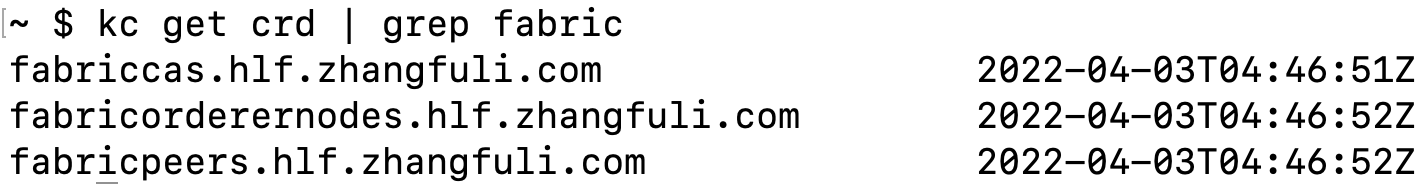
\includegraphics[width=0.9\textwidth]{FIGs/chapter5/crds.png} %中括号中的参数是设置图片充满文档的大小,你也可以使用小数来缩小图片的尺寸。
    \caption{CRD部署结果} %caption是用来给图片加上图题的
    \label{crdresult} %这是添加标签,方便在文章中引用图片。
\end{figure}%figure环境

\textbf{步骤一:} 如表\ref{org1_test}所示, HF网络管理员首先为org1创建了名为“org1-ca”的Ca节点; 其次, 在org1中创建了名为“org1-peer0”的Peer节点,并利用链外存储CouchDB作为账本存储单元。如图\ref{testcase1result}所示为测试结果。

{\footnotesize
\begin{longtable}[h]{m{45pt} m{45pt} m{180pt} m{50pt} m{20pt}}
    \caption[创建Org1测试用例]{Org1测试用例} \label{org1_test}\\
        \hline  
        用例编号&测试编号&用户输入&预期结果&实际\\
        \hline
        UC-Ca & TC1.1 & 创建名为org1-ca的Ca节点 & 成功启动Ca节点 & 通过 \\
        \hline
        UC-Peer & TC1.2 & 创建名为org1-peer0的Peer节点, 其拥有外部存储CouchDB, 所属于Org1MSP & 成功启动Peer节点 & 通过 \\
        \hline
    \end{longtable} 
}

\begin{figure}[h] %figure环境,h默认参数是可以浮动,不是固定在当前位置。如果要不浮动,你就可以使用大写float宏包的H参数,固定图片在当前位置,禁止浮动。
    \centering %使图片居中显示
    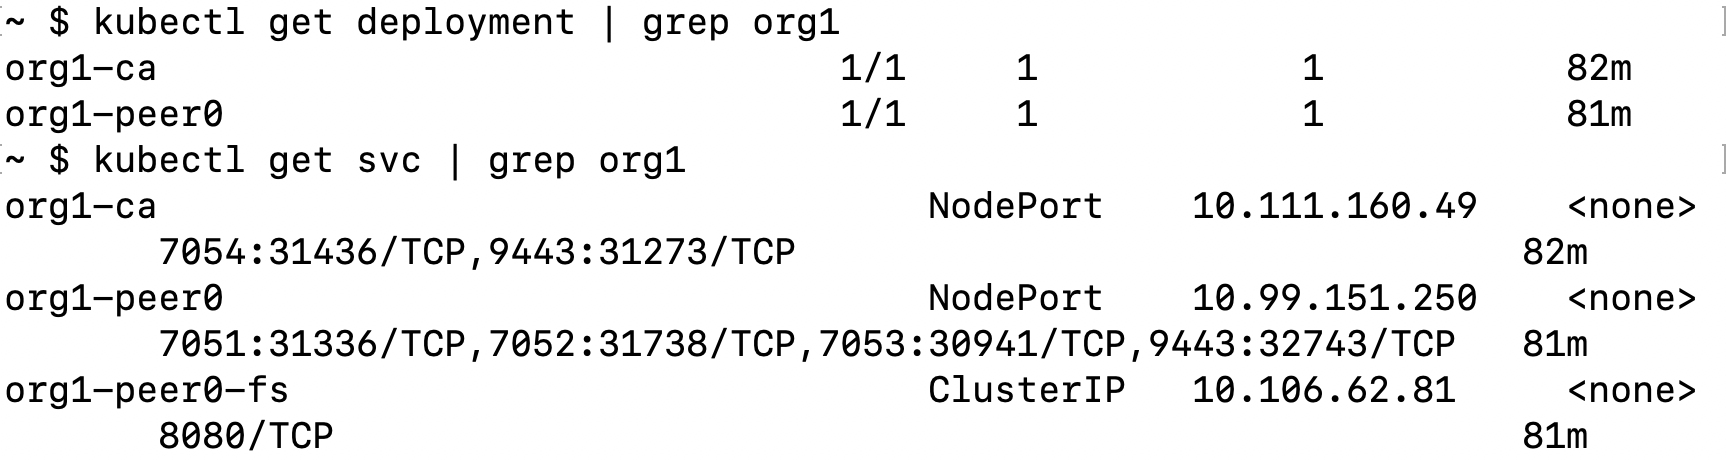
\includegraphics[width=0.9\textwidth]{FIGs/chapter5/peer.png} %中括号中的参数是设置图片充满文档的大小,你也可以使用小数来缩小图片的尺寸。
    \caption{创建Org1测试结果} %caption是用来给图片加上图题的
    \label{testcase1result} %这是添加标签,方便在文章中引用图片。
\end{figure}%figure环境

\textbf{步骤二:} 如表\ref{orderer_test}所示, HF网络管理员需要首先为OrdererMSP创建名为“ord-ca”的Ca节点; 其次, 在OrdererMSP中创建了名为“ord-node1”的Peer节点。如图\ref{testcase2result}所示为测试结果, 原型工具可以为HF网络管理员创建Orderer的Ca与Orderer节点, 其中包含但不限于Deployment、Service、Pod、Secret等。

{\footnotesize
\begin{longtable}[h]{m{45pt} m{45pt} m{180pt} m{50pt} m{20pt}}
    \caption[创建Orderer测试用例]{创建Orderer测试用例} \label{orderer_test}\\
        \hline  
        用例编号&测试编号&用户输入&预期结果&实际\\
        \hline
        UC-Ca & TC2.1 & 创建名为ord-ca的Ca节点 & 成功启动Ca节点 & 通过 \\
        \hline
        UC-Orderer & TC2.2 & 创建名为ord-node1的Orderer节点, 所属于OrdererMSP & 成功启动Orderer节点 & 通过 \\
        \hline
    \end{longtable} 
}

\begin{figure}[h] %figure环境,h默认参数是可以浮动,不是固定在当前位置。如果要不浮动,你就可以使用大写float宏包的H参数,固定图片在当前位置,禁止浮动。
    \centering %使图片居中显示
    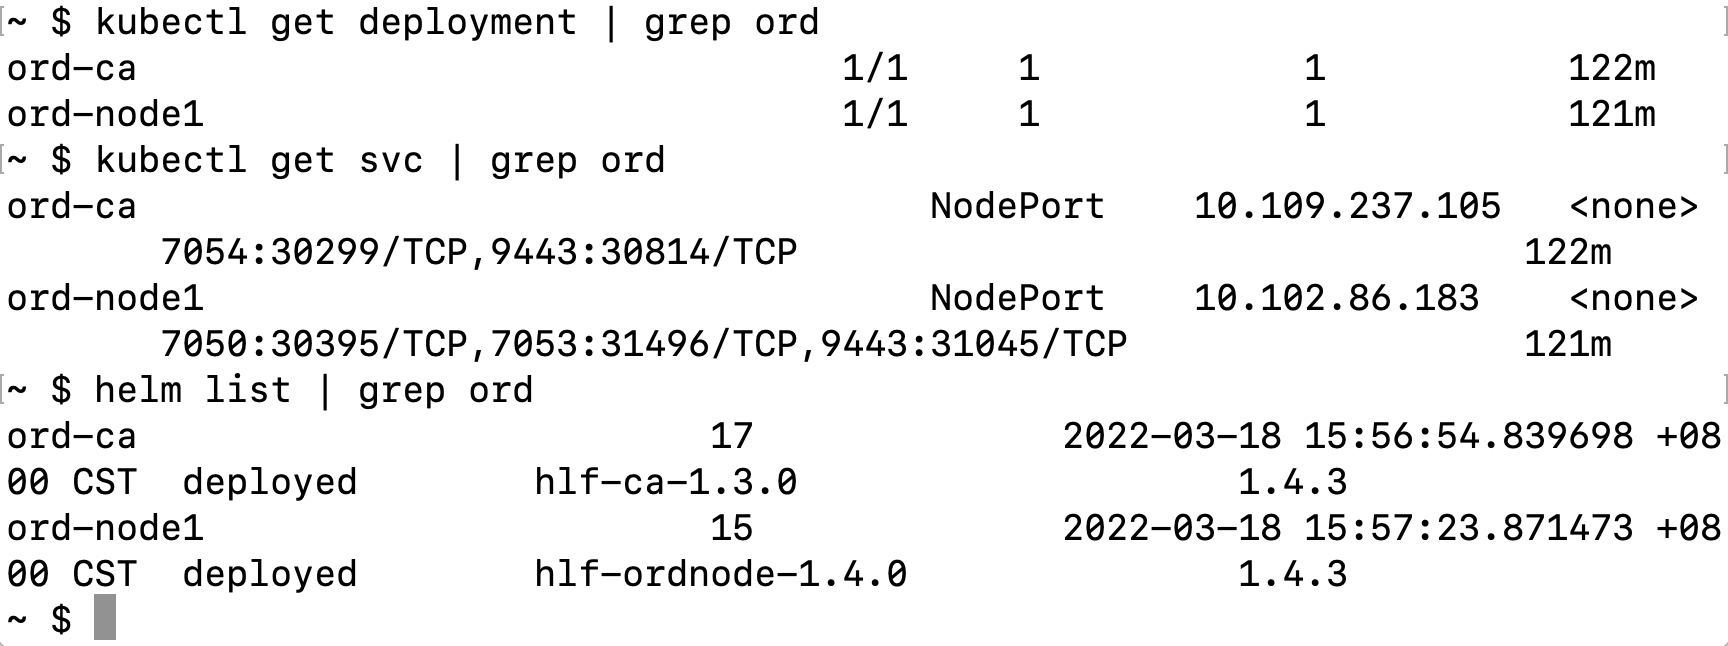
\includegraphics[width=0.9\textwidth]{FIGs/chapter5/orderer.png} %中括号中的参数是设置图片充满文档的大小,你也可以使用小数来缩小图片的尺寸。
    \caption{创建Orderer测试结果} %caption是用来给图片加上图题的
    \label{testcase2result} %这是添加标签,方便在文章中引用图片。
\end{figure}%figure环境

\textbf{步骤三:} 如表\ref{reg_enroll_test}所示, HF网络管理员需要为OrdererMSP以及Org1注册并登记若干用户, 并将用户的证书密钥信息导到yaml文件中。表中仅展示在Orderer中注册用户, Org1中步骤相似, 注册名为peeruser的用户。测试结果表明, 可以成功将用户及OrdererMSP信息导出。

\newpage

{\footnotesize
\begin{longtable}[h]{m{45pt} m{45pt} m{180pt} m{50pt} m{20pt}}
    \caption[注册、登记用户测试用例]{注册、登记用户测试用例} \label{reg_enroll_test}\\
        \hline  
        用例编号&测试编号&用户输入&预期结果&实际\\
        \hline
        UC-Ca & TC3.1 & 为OrdererMSP注册名为ordereruser的用户, 其密码为ordererpw & 成功注册 & 通过 \\
        \hline
        UC-Ca & TC3.2 & 输入用户名密码, 为ordereruser用户登记 & 成功登记,输出证书文件 & 通过 \\
        \hline
    \end{longtable} 
}

\textbf{步骤四:} 如表\ref{channel_test}所示, HF开发人员需要在新创建的HF网络上创建通道, 并初始化该通道内的创世区块。当通道被创建完成之后, 需要将在该通道内进行交易的的Orderer、Peer加入该通道。最后, HF开发人员可以指定锚节点并查看通道的高度。如图\ref{channel_test_result}所示为测试结果, 展示了新创建的通道的高度。

{\footnotesize
\begin{longtable}[h]{m{45pt} m{45pt} m{180pt} m{50pt} m{20pt}}
    \caption[创建通道测试用例]{创建通道测试用例} \label{channel_test}\\
        \hline  
        用例编号&测试编号&用户输入&预期结果&实际\\
        \hline
        UC-Chan & TC4.1 & 选择OrdererMSP为排序组织在Org1MSP上创建通道并创建创世节点 & 成功创建通道 & 通过 \\
        \hline
        UC-Orderer & TC4.2 & 将ord-node1加入通道 & 加入成功 & 通过 \\
        \hline
        UC-Peer & TC4.3 & 将org1-peer0加入通道 & 加入成功 & 通过 \\
        \hline
        UC-Chan & TC4.4 & 指定锚节点 & 指定成功 & 通过 \\
        \hline
        UC-Chan & TC4.5 & 查看通道高度 & 查看成功 & 通过 \\
        \hline
    \end{longtable} 
}

\begin{figure}[h] %figure环境,h默认参数是可以浮动,不是固定在当前位置。如果要不浮动,你就可以使用大写float宏包的H参数,固定图片在当前位置,禁止浮动。
    \centering %使图片居中显示
    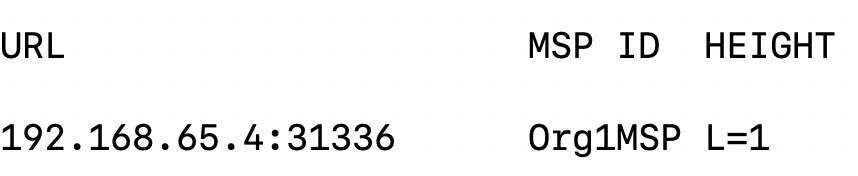
\includegraphics[width=0.55\textwidth]{FIGs/chapter5/channel.png} %中括号中的参数是设置图片充满文档的大小,你也可以使用小数来缩小图片的尺寸。
    \caption{查看通道高度测试结果} %caption是用来给图片加上图题的
    \label{channel_test_result} %这是添加标签,方便在文章中引用图片。
\end{figure}%figure环境

{\footnotesize
\begin{longtable}[h]{m{45pt} m{45pt} m{180pt} m{50pt} m{20pt}}
    \caption[创建通道测试用例]{创建通道测试用例} \label{chaincode_test}\\
        \hline  
        用例编号&测试编号&用户输入&预期结果&实际\\
        \hline
        UC-CC & TC5.1 & 安装链码并指定语言、label & 安装成功 & 通过 \\
        \hline
        UC-CC & TC5.2 & 查询已经安装的链码 & 查询成功 & 通过 \\
        \hline
        UC-CC & TC5.3 & 审批链码, 并提供链码ID以及策略 & 审批成功 & 通过 \\
        \hline
        UC-CC & TC5.4 & 提交链码, 并提供链码ID以及策略 & 指定成功 & 通过 \\
        \hline
        UC-CC & TC5.5 & 调用链码, 并提供链码调用函数 & 调用成功 & 通过 \\
        \hline
    \end{longtable} 
}

\textbf{步骤五:} 如表\ref{chaincode_test}所示, 为测试通道内所有的参与节点按照链码的合同规则执行, HF开发人员需要在新创建的通道内安装官方提供的asset\footnotemark[1]\footnotetext[1]{\href{https://github.com/hyperledger/fabric-samples/blob/main/asset-transfer-basic/chaincode-go/chaincode/smartcontract.go}{asset链码}}链码, 安装完链码之后, 需要对其进行审批、提交。最后, HF开发人员可以调用链码接口对其进行初始化、查询等一系列操作。如图\ref{chaincode_test_result}所示为测试结果, 展示了查询链码之后的结果。

\begin{figure}[h] %figure环境,h默认参数是可以浮动,不是固定在当前位置。如果要不浮动,你就可以使用大写float宏包的H参数,固定图片在当前位置,禁止浮动。
    \centering %使图片居中显示
    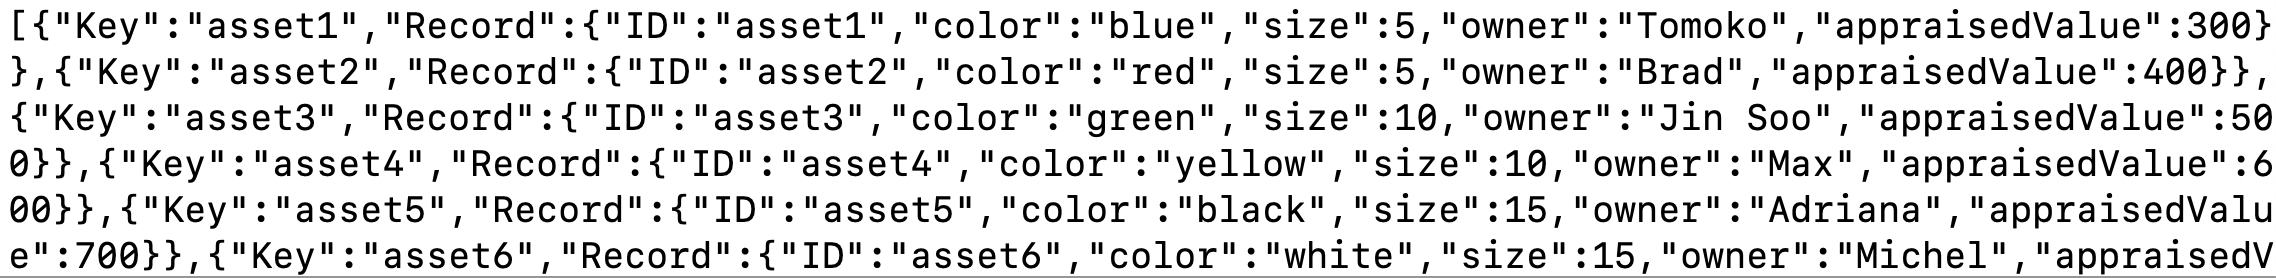
\includegraphics[width=1.0\textwidth]{FIGs/chapter5/chaincode.png} %中括号中的参数是设置图片充满文档的大小,你也可以使用小数来缩小图片的尺寸。
    \caption{查询链码} %caption是用来给图片加上图题的
    \label{chaincode_test_result} %这是添加标签,方便在文章中引用图片。
\end{figure}%figure环境


经过上述步骤1-5, 最终的网络节点状态如图\ref{fabric_result}所示, 本文搭建了一个单Orderer以及单Org、单Peer的简单的HF网络, 并分别Orderer、以及Peer搭配Ca证书认证。在搭建了基本的网络之后, 分别为Orderer、Peer注册并登记用户, 最后在组织Org中搭建了一个通道并成功安装调用链码。测试结果可知, 本文的原型工具能够正常成功搭建HF网络及部署链码。


\begin{figure}[h] %figure环境,h默认参数是可以浮动,不是固定在当前位置。如果要不浮动,你就可以使用大写float宏包的H参数,固定图片在当前位置,禁止浮动。
    \centering %使图片居中显示
    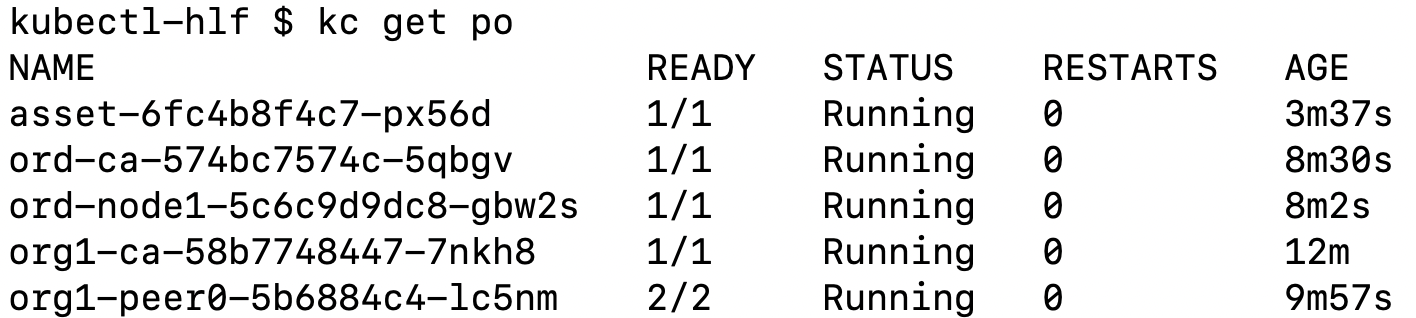
\includegraphics[width=1.0\textwidth]{FIGs/chapter5/fabric_result.png} %中括号中的参数是设置图片充满文档的大小,你也可以使用小数来缩小图片的尺寸。
    \caption{网络节点状态} %caption是用来给图片加上图题的
    \label{fabric_result} %这是添加标签,方便在文章中引用图片。
\end{figure}%figure环境

\section{原型工具评估}

\subsection{架构评估}

在软件工程中, 常见的评估软件体系结构的方法有Software Architecture Analysis Method(SAAM)、Architecture Trade-off Analysis Method(ATAM), 以上都是基于场景的质量属性评估方法\cite{ionita2002scenario}。SAAM相较于ATAM而言其结构以及评估过程相对简单, 需要准备的工作较少并且SAAM适用于对软件最终版本的评估\cite{huhonglei2004}。本文首先对第\ref{section: framework_characteristics}节所涉及到的设计原则的描述映射到对应的质量属性, 然后采取SAAM方法对其进行评估。

在SAAM评估方法开始之前, 本文邀请了4位熟悉HF基本概念及网络搭建流程的软件开发工程师分别两两扮演HF网络管理员、HF开发人员, 1位熟悉Kubernetes操作的集群运维工程师扮演集群管理员, 以上5位分别为本次SAAM评估方法的风险承担者。本节实施SAAM评估方法涉及以下步骤:

\textbf{1. 场景开发: }所有的风险承担者通过头脑风暴的方式, 提出反应自己需求的场景, 产出结果见步骤3。

\textbf{2. 软件架构描述: }本文详细的为各位风险承担者介绍第四节的面向Hyperledger Fabric的区块链云化框架及其原型工具, 包括框架设计理念与原理、原型工具功能与工具实现结构。

\textbf{3. 场景分类: }在这个过程中, 如表\ref{saam_step3}所示, 本文对步骤1所产出的场景进行分类并设定优先级。同时, 在分析时根据场景是否需要修改特定的体系结构把场景分为直接场景与间接场景。

{\footnotesize
\begin{longtable}[h]{m{20pt} m{60pt} m{90pt} m{40pt} m{40pt} m{40pt} m{30pt}}
    \caption[场景分类结果]{场景分类结果} \label{saam_step3}\\
        \hline  
        编号&风险承担者&场景描述&设计原则 & 质量属性 & 场景分类 & 优先级\\
        \hline
        T1&  HF网络管理员 & 命令式启停HF网络中的任意节点 & 简单易用  & 功能需求 & 直接需求 &  高 \\
        \hline
        T2&  HF网络管理员 & 命令创建HF网络用户 & 简单易用 & 功能需求 & 直接需求 &  高 \\
        \hline
        T3&  HF开发人员 & 命令式创建通道 & 简单易用 & 功能需求 & 直接需求 &  高 \\
        \hline
        T4&  HF开发人员 & 命令式操作链码 & 简单易用 & 功能需求 & 直接需求 &  高 \\
        \hline
        T5&  HF网络管理员 \newline HF开发人员 & 能在30min内启动完整网络 & 简单易用 & 易用性 & 间接需求 &  高 \\
        \hline
        T6&  HF网络管理员 & 扩容HF节点资源 & 灵活扩展 & 可扩展性 & 间接需求 &  中 \\
        \hline
        T7&  HF网络管理员 & 扩容账本存储单元 & 灵活扩展 & 可扩展性 & 间接需求 &  高 \\
        \hline
        T8&  HF开发人员 & 保存用户密钥 & 安全可靠 & 安全性 & 间接需求 &  高 \\
        \hline
        T9&  HF开发人员 & 操作网络时需要身份认证 & 安全可靠 & 安全性 & 间接需求 &  高 \\
        \hline    
        T10&  k8s管理员 & HF网络与其他集群程序进行隔离 & 安全可靠 & 安全性 & 间接需求 &  高 \\
        \hline
        T11&  k8s管理员 & Operator限定管理HF网络节点 & 安全可靠 & 安全性 & 间接需求 &  高 \\
        \hline
        T12&  HF网络管理员 \newline HF开发人员 & 良好异常反馈机制 & 安全可靠 & 可靠性 & 间接需求 &  高 \\
        \hline
        T13&  HF网络管理员 \newline HF开发人员 & HF网络节点的全面监控能力 & 可视运维 & 可靠性 & 间接需求 &  高 \\
        \hline
        T14&  HF网络管理员 \newline HF开发人员 & Operator在不同云平台之间迁移的便捷性 & 云链结合 & 可移植性 & 间接需求 &  中 \\
        \hline
    \end{longtable} 
}

\textbf{4. 场景评估: }这个过程重点针对间接场景, 并对其进行评估。针对直接场景, 第\ref{section: tool_test}节已经对其进行了较为全面的功能性测试。

简单易用, 本文同时邀请了这5位风险承担者对本文的原型工具进行易用性测试。为了排除网络的影响,
本文提前下载好原型工具搭建HF网络所需要的Docker镜像。在介绍了本工具的基本原理以及命令行的基本使用方法后, 5位风险承担者分别独立自行搭建不同规格的HF网络, 最终5位风险承担者都能够在30分钟内学习并掌握原型工具的使用方法。

灵活扩展, 在HF网络节点资源方面, 由于HF网络节点的CRs中配置了HF网络节点运行态时所需的资源(CPU、Mem)大小, 所以当对节点CR进行修改时, Controller会监听到CR的变化并更新运行中节点Deployment的资源大小。在数据存储的可扩展性方面,如图\ref{db}所示, 原型工具为每个HF网络中的工作节点设置了专属存储单元。每个存储单元配置专属的PVC管理, HF网络管理员可以不仅可以通过修改节点的CRs进行扩容, 可以直接在Kubernetes中对PVC进行动态扩容。值得注意的是, 由于存储单元PVC扩容依赖于StorageClass, 当前只有AWS-EBS、GCE-PD、Azure磁盘、Azure文件、Glusterfs、Cinder、Portworx和Ceph RBD数据卷插件才能支撑数据扩容操作。

\begin{figure}[h] %figure环境,h默认参数是可以浮动,不是固定在当前位置。如果要不浮动,你就可以使用大写float宏包的H参数,固定图片在当前位置,禁止浮动。
    \centering %使图片居中显示
    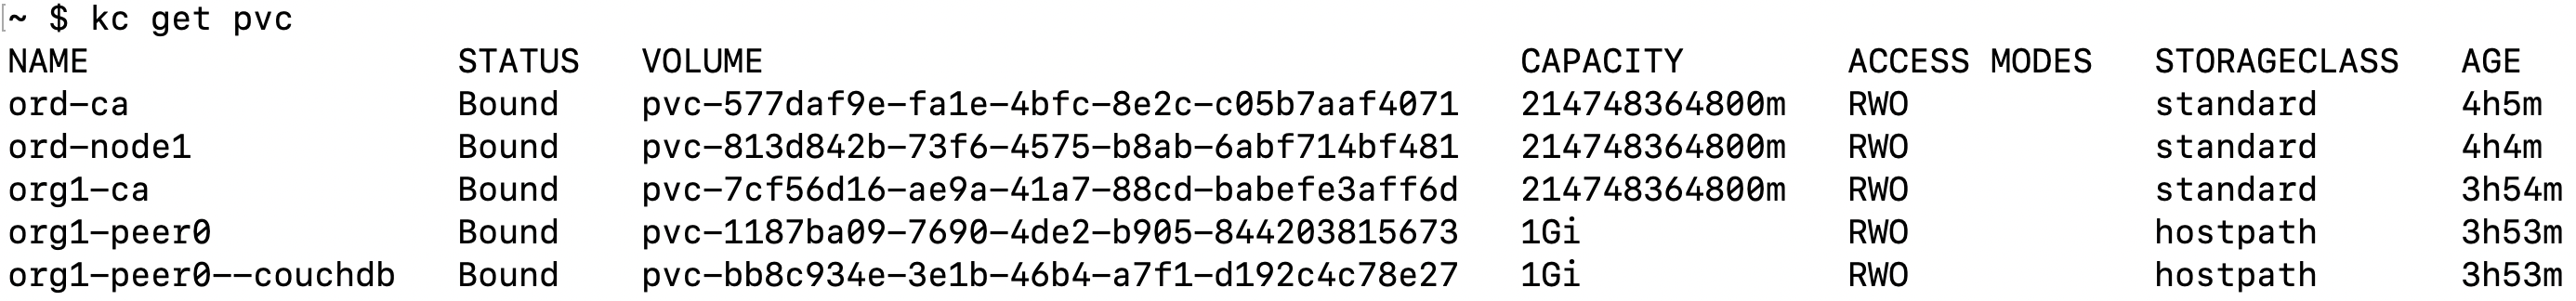
\includegraphics[width=1.0\textwidth]{FIGs/chapter5/db.png} %中括号中的参数是设置图片充满文档的大小,你也可以使用小数来缩小图片的尺寸。
    \caption{网络存储状态} %caption是用来给图片加上图题的
    \label{db} %这是添加标签,方便在文章中引用图片。
\end{figure}%figure环境

安全可靠, 原型工具通过可以以文件形式导出HF网络登记用户产生的密钥信息, 并可以通过Secret进行保存。当这些用户操作HF网络时, 原型工具会要求提供对应的密钥文件作为身份认证的方式。同时, 原型工具将所有的HF资源放在同一命名空间下, 并通过RBAC为该命名空间提供了两种类型的角色。当集群其他用户对已经部署的HF网络节点拥有超越权限的操作时, 原型工具会提示并不进行相关操作。在可靠性方面, 本文在使用原型工具搭建HF网络过程中有意输入错误的命令行参数, 输入不正确的密钥文件等, 原型工具都能在1s内给出参数的异常情况; 同时, 原型工具能够有效利用Prometheus监控体系对工具本身以及HF网络的所有节点、智能合约以及DB进行监控, 如图\ref{monitoring}展示了利用Prometheus与Grafana对Fabric Ca Resource进行监控的画面, 图中展示了Fabric Ca Resource的API、内存以及CPU的使用情况。在搭建完HF网络之后, 原型工具在两周内仅崩溃1次, 且能通过日志以及Prometheus的告警设置在5分钟内进行恢复。

云链结合, 重点是在可移植性下的场景。本文通过Dockerfile将本工具打包成Docker镜像\footnotemark[1]\footnotetext[1]{\href{https://hub.docker.com/repository/docker/zhangfuli/hfoperator}{HFOperator镜像}}, 使用预先打包并经过检验的镜像, 并为该原型工具配备专用的Helm chart, 其中包含有关原型工具构建的所有必要信息, 这样可以以最少的时间部署。结果表明, 原型工具可以通过Helm在支持Kubernetes 1.18版本以上的云平台上运行, 原型平台具备良好的可移植性性。

\begin{figure}[h] %figure环境,h默认参数是可以浮动,不是固定在当前位置。如果要不浮动,你就可以使用大写float宏包的H参数,固定图片在当前位置,禁止浮动。
    \centering %使图片居中显示
    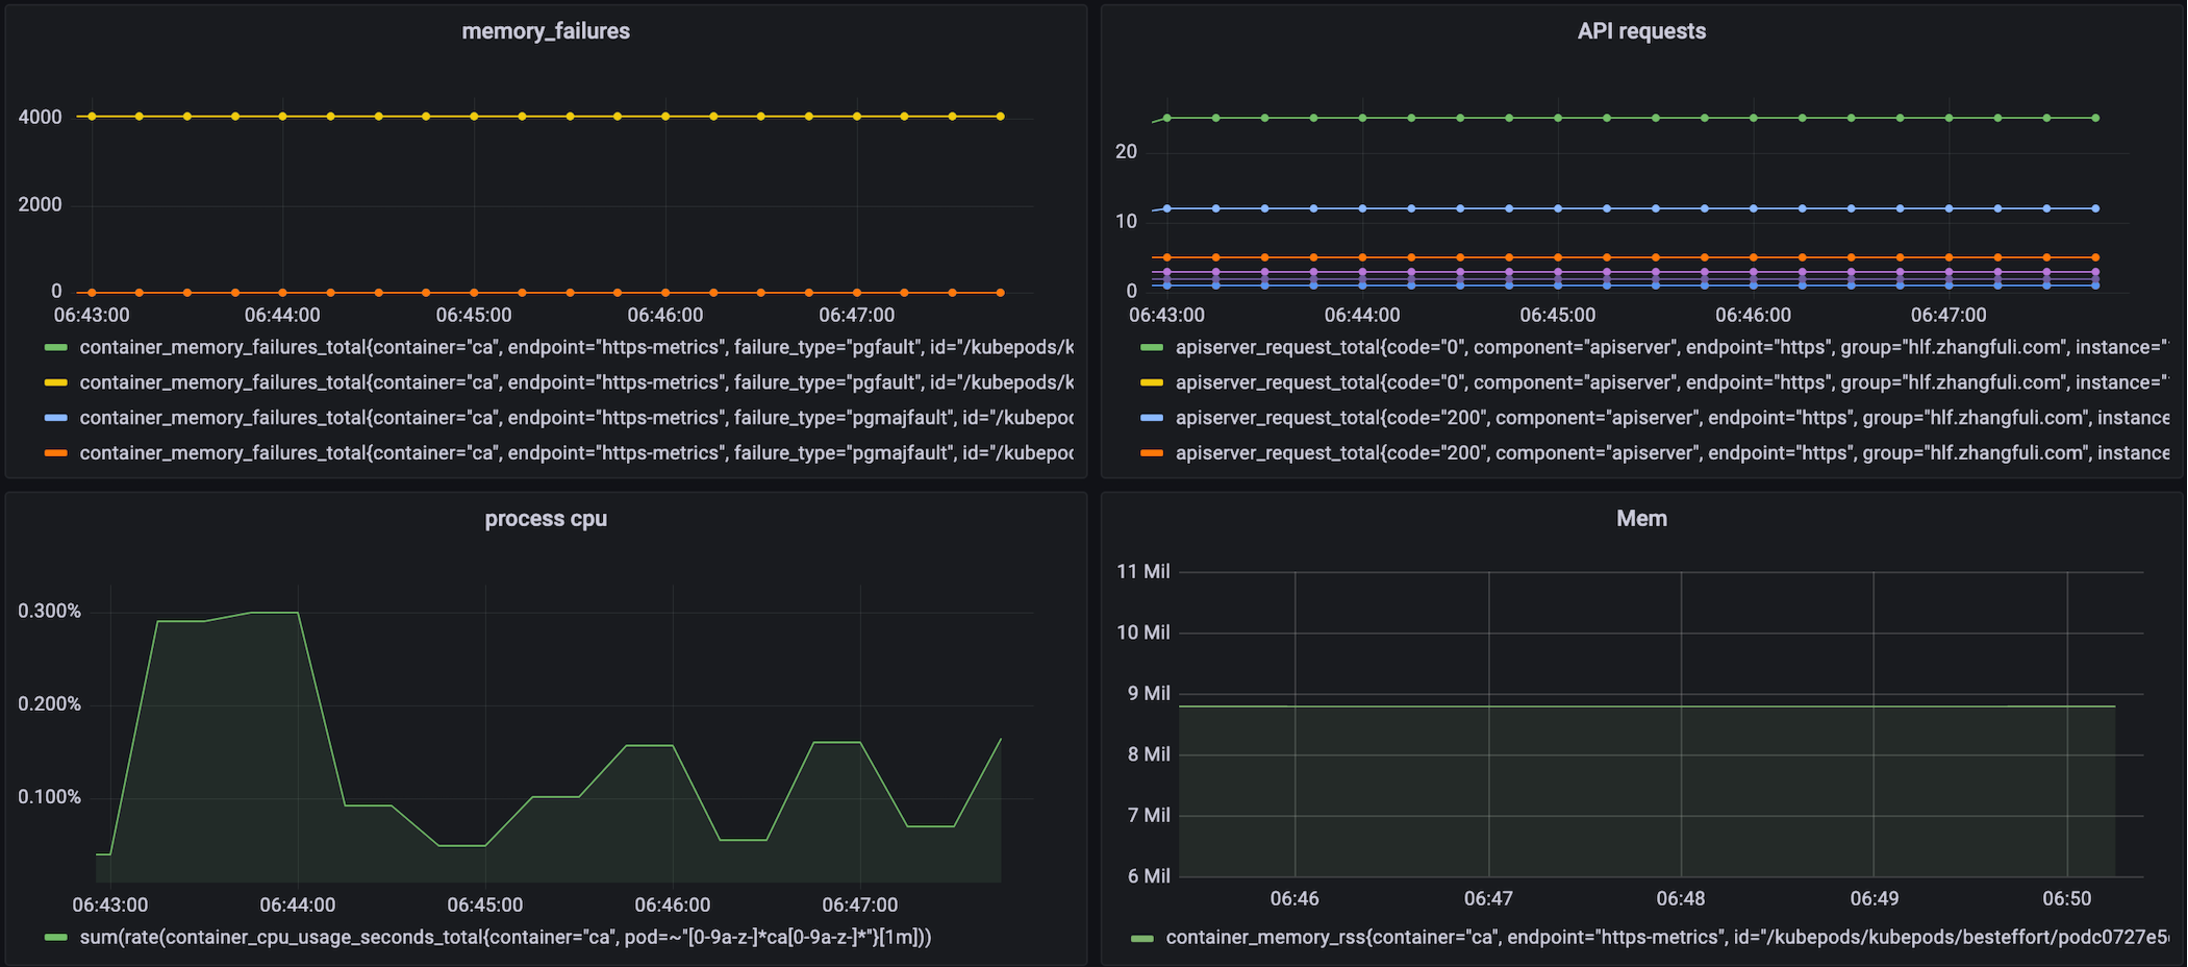
\includegraphics[width=0.9\textwidth]{FIGs/chapter5/monitoring.pdf} %中括号中的参数是设置图片充满文档的大小,你也可以使用小数来缩小图片的尺寸。
    \caption{Fabric Ca Resource监控图} %caption是用来给图片加上图题的
    \label{monitoring} %这是添加标签,方便在文章中引用图片。
\end{figure}%figure环境

\textbf{5. 总体评估: }本文的原型工具可以有效利用Kubernetes Operator云化策略来提升HF网络的易用性、可扩展性、安全性、以及可靠性。


\subsection{五层成熟度模型}

如图所示\ref{maturity}, Kubernetes Operator拥有5个成熟度级别的定义\cite{duan2021case}, 其通过定性的方式分析某个Operator应用是否达到了某个级别, 这5个成熟度级别定义如下:

\begin{itemize}[itemindent=2em]
    \item 第一级: Basic Intall, 该级是Operator成熟度模型中最基本的级别。在该级中, 用户能够使用CRD对目标程序进行配置和安装;

    \item 第二级: Seamless Upgrades, 在该级别上的Operator能够不丢失数据的升级所管理的工作负载;

    \item 第三级: Full Lifecycle, 是否能达到该级别取决于Operator是否具备生命周期管理和的数据备份、恢复能力。在该级别上的Operator能够备份数据, 并在发生任何数据灾难时从备份数据中恢复数据。

    \item 第四级: Deep Insights, Operator提供监控和报警等功能。在该级别, Operator能够包含所有组件的运行状况指标, 并根据指标配备报警功能;

    \item 第五级: Auto Pilot, 最终级别拥有许多高级功能, 如自动伸缩。Operator可以通过收集到的指标来扩展工作负载。

\end{itemize}

\begin{figure}[h] %figure环境,h默认参数是可以浮动,不是固定在当前位置。如果要不浮动,你就可以使用大写float宏包的H参数,固定图片在当前位置,禁止浮动。
    \centering %使图片居中显示
    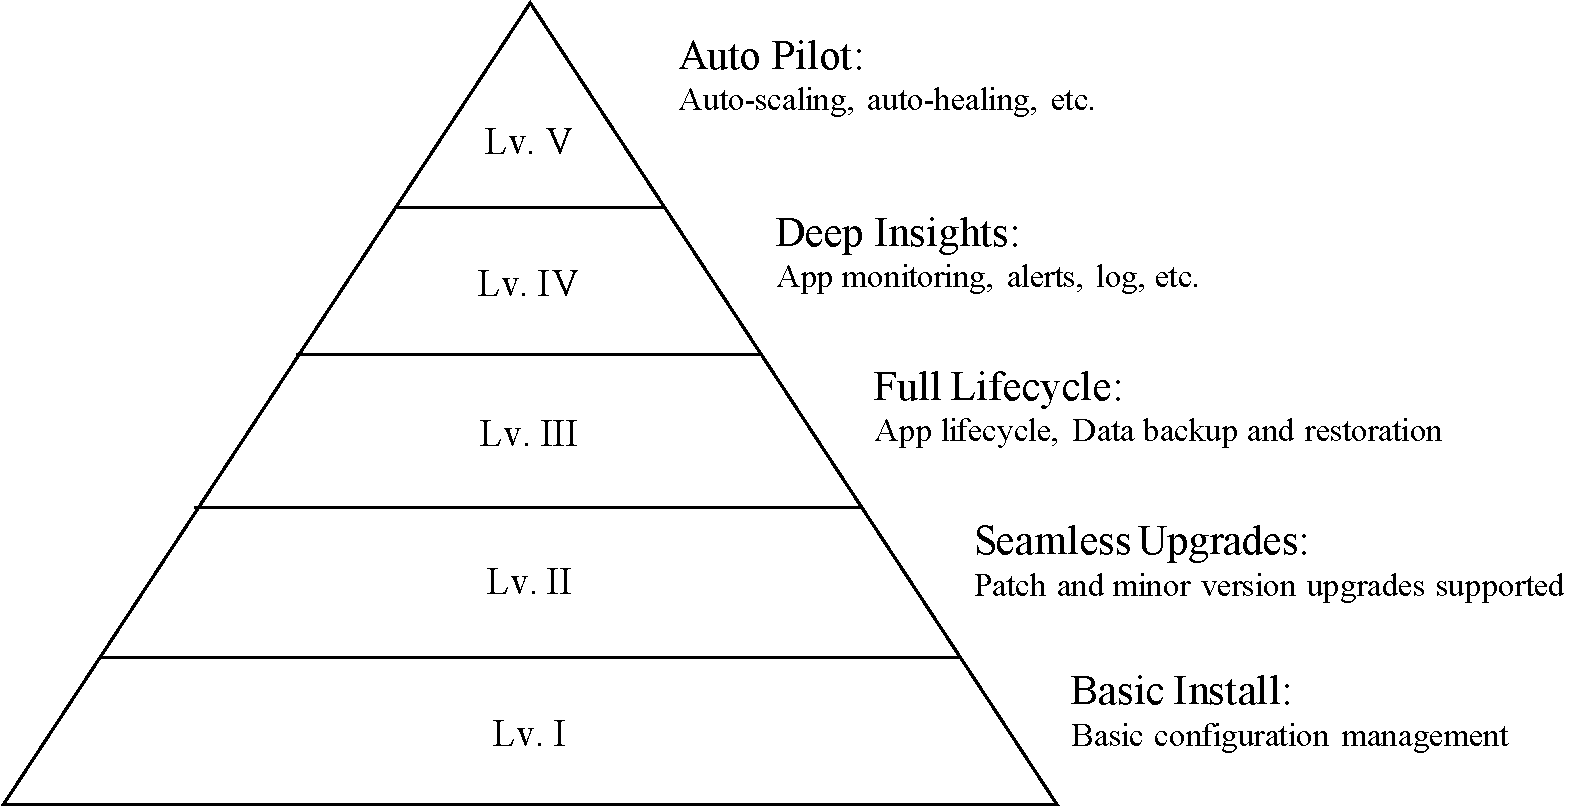
\includegraphics[width=0.9\textwidth]{FIGs/chapter5/maturity.pdf} %中括号中的参数是设置图片充满文档的大小,你也可以使用小数来缩小图片的尺寸。
    \caption{成熟度模型} %caption是用来给图片加上图题的
    \label{maturity} %这是添加标签,方便在文章中引用图片。
\end{figure}%figure环境

\textbf{Basic Install}

借助于原型工具, 能够通过命令行方式一键启停HF网络中任意节点, 而且不需要进行复杂的证书管理。一旦原型工具被部署在Kubernetes网络中, 原型工具就可以对CRs以及Helm进行管理, HF网络管理人员可以借助命令行参数的方式进行创建、更新CRs以此来创建特定规格的HF网络。 一旦CRs进行更新, 原型工具就会将当前状态调整为与指定状态一致。

\textbf{Seamless Upgrades}

在原型工具中, HF网络管理员可以通过修改CRs的内容对包括HF网络节点镜像、端口、host、版本等进行无缝修改。此外, 由于原型工具依赖于链外存储的CouchDB, 以及外部的Prometheus监控体系, 这两者的升级并不会对原型工具产生严重的负面影响。 

\textbf{Full Lifecycle}

虽然原型工具能够在Mangager中对结合Helm对HF网络进行全生命周期管理, 但目前原型工具目前仍缺少数据备份和恢复的能力。要达到这一能力需要在CRs中指定远程备份的数据存储平台, 并在CRs中指定数据备份的凭证以及远程备份的链接。同时, 原型工具需要在一定的时间周期内将数据备份的到远程的数据存储平台上。

\textbf{Deep Insights}

原型工具利用Prometheus监控体系实现监控与报警的功能, 与此同时, 除了让Prometheus抓取Pod的基本指标外, CRD中还设定了PodMonitor、ServiceMonitor、CouchDBExporter接口, 可以让Prometheus更全面的抓取HF网络的监控指标。HF网络管理员可以通过Grafna可视化图表查看整体HF网络运行状态, 并且能够根据监控指标创建自定义的告警规则。

\textbf{Auto Pilot}

在Kubernetes中存在两种自动伸缩的插件, 即HPA、VPA。当负载超过一定的阈值时, 就会对其进行伸缩或配置更多的资源。然而在HF网络中, 每个Peer都有记录全部账本的职责, 并且只需要超过51\%的Peer节点保持一致即可, 所以针对于Peer并不需要根据监控进行自我伸缩的能力。在数据存储方面, 随着账本的膨胀, 原型工具可以针对链外存储进行扩容。

综上, 通过定性分析, 本文原型工具利用Operator管理HF网络能够完美的具备第一级、第二级在第三级上能够支持全生命周期管理但是对于数据的备份能力依旧是存在欠缺, 借助原型工具实现了第四级的监控, 对于自动伸缩方面支持资源及数据层面的扩展, 所以本文原型工具基本满足5层成熟度模型的功能。

\subsection{工具对比} \label{section: tool_comparison}

除上述通过定性分析的手段对运行工具进行评估外, 本文选取了Hyperledger官方推出的BaaS平台Cello进行定量数据的对比分析。本文重点关注的是对HF网络节点的云化问题, 所以需要在网络部署时间上对Cello以及原型工具进行对比。

本文在云主机环境下拉取Cello的release-0.9.0-h3c并进行打包构建以及运行。Cello通过图形化的Cello Operator进行主机绑定、组织管理、网络管理以及用户管理。操作Cello Operator的就是HF网络管理员, 管理员首先在主机管理中添加主机, 主机就是Cello将要部署的目标Docker或者Kubernetes环境, 然后再依次创建组织并启动网络, 整个过程全都通过图形化界面的方式完成。

% 如图\ref{cello}所示,
% \begin{figure}[h] %figure环境,h默认参数是可以浮动,不是固定在当前位置。如果要不浮动,你就可以使用大写float宏包的H参数,固定图片在当前位置,禁止浮动。
%     \centering %使图片居中显示
%     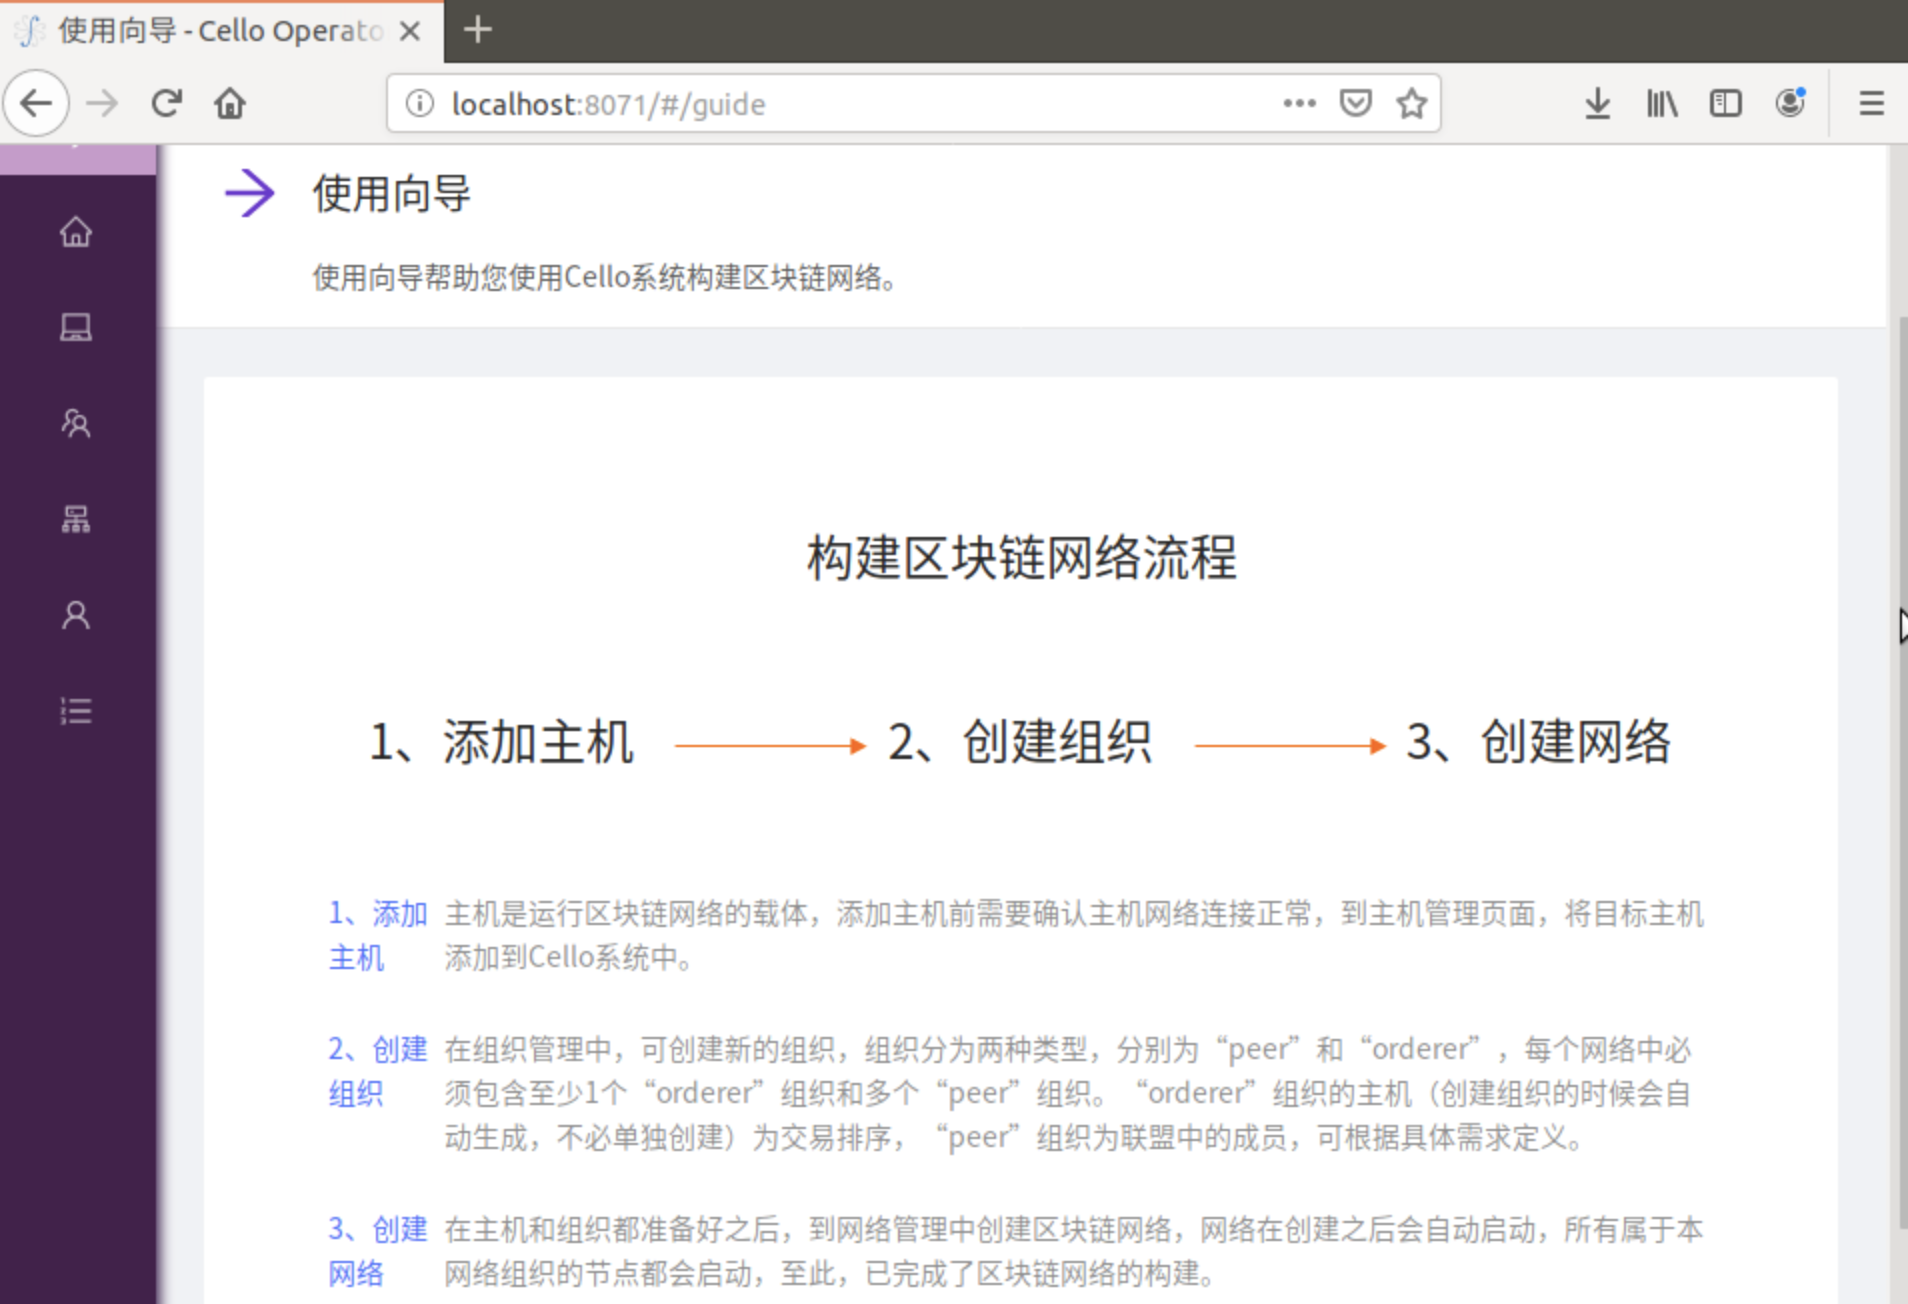
\includegraphics[width=0.95\textwidth]{FIGs/chapter5/cello.png} %中括号中的参数是设置图片充满文档的大小,你也可以使用小数来缩小图片的尺寸。
%     \caption{图形化Cello Operator} %caption是用来给图片加上图题的
%     \label{cello} %这是添加标签,方便在文章中引用图片。
% \end{figure}%figure环境


{\footnotesize
\begin{longtable}[h]{m{100pt} m{100pt} m{100pt}}
    \caption[Hyperledger Fabric版本信息]{Hyperledger Fabric版本信息} \label{test_fabric_net} \\
        \hline  
        \textbf{镜像}&\textbf{Cello版本}&\textbf{原型工具版本}\\
        \hline
        Fabric-Ca & 1.4.2 & 1.4.9 \\
        Fabric-Peer & 1.4.2 & 2.4.1 \\
        Fabric-Orderer & 1.4.2 & 2.4.1 \\
        \hline
    \end{longtable}
}

由于现在在Docker环境中部署HF网络仍旧是主流, 所以本文利用Cello在Docker中部署作为测试基准。由于Cello的局限性, 仅支持在部署HF网络的1.4版本, 而原型工具能更优的支持HF网络的2.X以上版本。
如表\ref{test_fabric_net}展示了本次工具对比所部署的HF网络各节点的版本信息, 测试基准为基于单组织单Peer的网络部署时间, 共识算法选择Solo, 数据存储选择LevelDB。


为了避免人为的手工干扰, 获得更加准确的网络部署时间。本文提前在Cello Operator中创建好Orderer以及org1组织并为每个组织配置一个对应的节点。当点击提交网络时开始计时, 刚开始创建时, 网络节点的状态是“故障”, 当网络节点的状态从“故障”变成“正常”时停止计时, 随后删除该网络。重复10次上述操作, 且为避免后端镜像遗留干扰, 每次操作间隔3min~5min。在原型工具中, 为避免手工输入命令而带来的人为误差, 本文预先编写好创建网络的脚本, 脚本中创建10次网络, 创建完成后删除该网络并在删除后休眠30s, 如此循环10次共得到10次网络启动时间如表\ref{net_deployment_time}所示。

{\footnotesize
\begin{longtable}[h]{m{35pt}|m{40pt}|m{15pt} m{15pt} m{15pt} m{15pt} m{15pt} m{15pt} m{15pt} m{15pt} m{15pt} m{15pt}|m{20pt}}
    \caption[网络部署时间(单位: 秒(s))]{网络部署时间(单位: 秒(s))} \label{net_deployment_time}\\
        \hline
        \multirow{2}*{工具类型}
        & \multirow{2}*{\parbox[c]{40pt}{节点类型}}
        & \multicolumn{10}{c|}{序号}
        
        & \multirow{2}*{\parbox[c]{20pt}{平均}}\\
        \cline{3-12}
        & & 1 & 2 & 3 & 4 & 5 & 6 & 7 & 8 & 9 & 10 & \\
        \hline
        Cello & 整体网络 & 73 & 119 & 115 & 90 & 73 & 89 & 137 & 85 & 103 & 127 & 101.1\\
        \hline  
        \multirow{5}*{\parbox[c]{40pt}{原型工具}}
        & ca(peer) & 13 & 12 & 13 & 13 & 13 & 13 & 13 & 12 & 12 & 12 & 12.6 \\
        & peer & 20 & 21 & 29 & 16 & 23 & 27 & 20 & 20 & 16 & 22 &  21.4 \\
        & ca(ord) & 13 & 13 & 13 & 13 & 13 & 13 & 14 & 13 & 15 & 15 & 13.5 \\
        & orderer & 27 & 36 & 34 & 24 & 33 & 24 & 27 & 25 & 32 & 25 & 28.7 \\
        \cline{2-13}
        & 整体网络 & 73 & 82 & 89 & 66 & 82 & 77 & 74 & 70 & 75 & 74 & 76.2\\
        \hline
    \end{longtable} 
}

\begin{figure}[h] %figure环境,h默认参数是可以浮动,不是固定在当前位置。如果要不浮动,你就可以使用大写float宏包的H参数,固定图片在当前位置,禁止浮动。
    \centering %使图片居中显示
    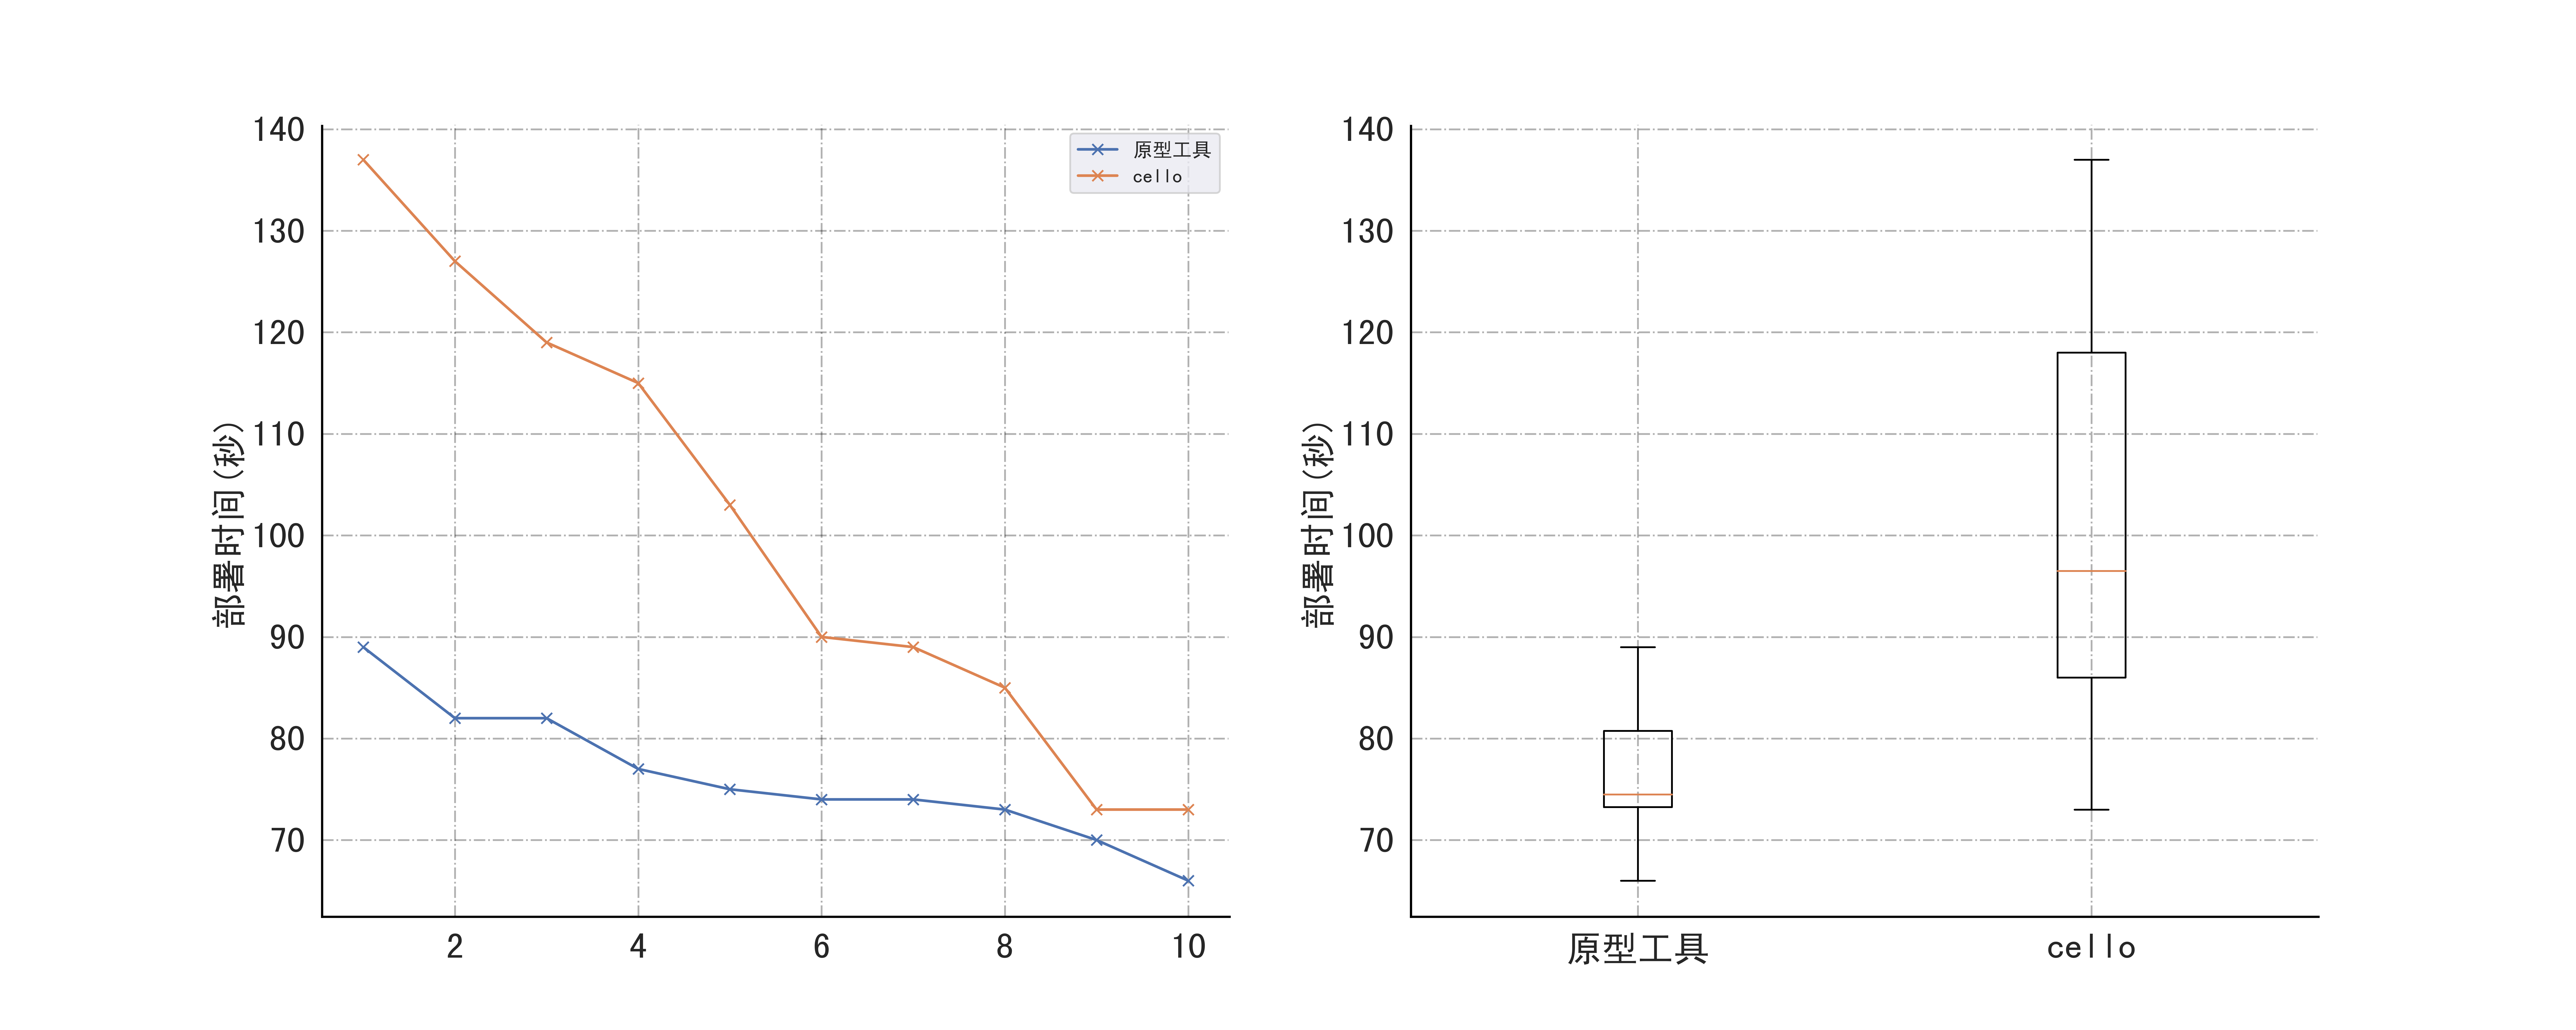
\includegraphics[width=1.0\textwidth]{FIGs/chapter5/plt_deployment.png} %中括号中的参数是设置图片充满文档的大小,你也可以使用小数来缩小图片的尺寸。
    \caption{网络部署时间对比图} %caption是用来给图片加上图题的
    \label{plt_deployment} %这是添加标签,方便在文章中引用图片。
\end{figure}%figure环境

如图\ref{plt_deployment}展示了原型工具和Cello分别部署HF网络的对比图。值得注意的是, 由于Cello采用图形化界面无法单独配置单个Ca的启停, 所以采用Cello部署的单Orderer单组织的HF网络仅在单个组织内部启动了一个Ca节点, 共计3个网络节点。 而采用原型工具部署的单Orderer单组织的HF网络分别为Orderer以及单组织部署了一个Ca节点, 共计4个网络节点。图\ref{plt_deployment}左侧展示了对着10次部署排序后的时间曲线图, 图中可以较为直观的看到原型工具比Cello部署的时间要少, 原型工具的部署整体网络的平均时间为76.2秒, 而Cello部署整体网络的平均时间为101.1秒; 经计算, 原型工具的总体标准偏差约为6.29, Cello的总体标准偏差约为21.41。图\ref{plt_deployment}右侧分别展示了两者的箱线图, 结合标准偏差可知原型工具部署时间相对而言更为稳定, 尤其在部署Ca节点时, 稳定在13秒左右。

通过分析源码\footnotemark[1]\footnotetext[1]{\href{https://github.com/hyperledger/cello/blob/release-0.9.0-h3c/src/modules/blockchain_network.py}{cello create network}}可知, 当在Cello Operator前端中提交网络之后, Cello对应的Docker Agent会循环解析传入的HF网络节点信息及数量的数据结构, 解析完成后串行构建HF网络中的各类节点。构建过程中, 采用生成Docker Compose文件并启动对应的网络节点。同样, 当Cello选择在Kubernetes部署时根据Template模板在代码中硬编码生成yaml文件。由此可得, Cello网络部署时间会随着HF网络中节点数量的增加而线性递增。本文的原型工具, 因需要手动以命令的方式部署单个对应网络节点, 其部署时间也会随着节点数量增加而递增。因此, 只对单Orderer单Peer进行对比测试即可预估出不同网络规模下的网络部署时间。

综上, 通过定量分析, 本文原型工具相较于Cello在具有更优的部署时间, 并且每次部署时间更加稳定。

% 链码调用时间
% 数据落盘时间
% 数据读取能力

\section{本章小结}

本章介绍了对原型工具的测试与评估。首先介绍了本文涉及到的两个测试环境, 并以典型案例的方式对原型工具进行了功能性测试, 最终的测试符合预期。其次, 本章利用SAAM、定性与定量的方法, 分别对原型工具进行了评估。
